\documentclass[tikz,border=3pt]{standalone}
\usepackage{amsmath}
\usepackage{tikz}
\usetikzlibrary{arrows.meta}
\begin{document}
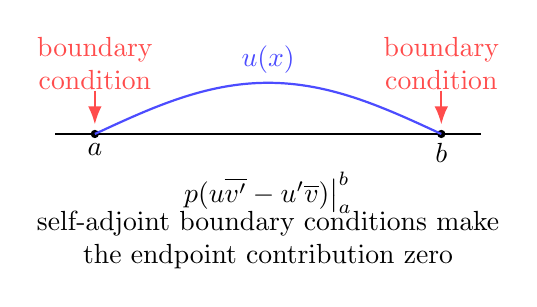
\begin{tikzpicture}[>=Latex,scale=1.0]
  \draw[thick] (-2.7,0) -- (2.7,0);
  \fill (-2.2,0) circle (1.5pt) node[below] {$a$};
  \fill (2.2,0) circle (1.5pt) node[below] {$b$};
  \draw[blue!70,thick,domain=-2.2:2.2,samples=120]
    plot (\x,{0.65*sin(180*(\x+2.2)/4.4)});
  \node[blue!70,above] at (0,0.65) {$u(x)$};
  \node at (0,-0.75) {$p(u\overline{v'}-u'\overline v)\big|_a^b$};
  \draw[->,red!70,thick] (-2.2,0.55) -- (-2.2,0.12);
  \draw[->,red!70,thick] (2.2,0.55) -- (2.2,0.12);
  \node[red!70,align=center] at (-2.2,0.9) {boundary\\condition};
  \node[red!70,align=center] at (2.2,0.9) {boundary\\condition};
  \node[align=center] at (0,-1.35) {self-adjoint boundary conditions make\\the endpoint contribution zero};
\end{tikzpicture}
\end{document}
